\documentclass[conference]{IEEEtran}

\usepackage{cite}
\usepackage{amsmath,amssymb,amsfonts}
\usepackage{algorithmic}
\usepackage{algorithm}
\usepackage{booktabs}
\usepackage{graphicx}
\usepackage{textcomp}
\usepackage{xcolor}
\usepackage{tikz}
\usepackage{pgfplots}
\usepackage[hidelinks]{hyperref}
\usepackage{orcidlink}
\usetikzlibrary{arrows.meta,positioning}
\usepackage{balance}
\pgfplotsset{compat=1.15}
\newcommand{\CalibratedPimOverheadFour}{0.118}
\newcommand{\CalibratedPimOverheadSixtyFour}{0.118}
\newcommand{\CalibratedPimZeroOverheadFour}{0.048}
\newcommand{\NativeComputeLanes}{0}
\newcommand{\NativeDmaBurstKiB}{0}
\newcommand{\NativeGateStatus}{passed}
\newcommand{\NativeMeanTicks}{2104955000}
\newcommand{\NativePipelineBuffers}{0}
\newcommand{\NativeRowCount}{36}
\newcommand{\NativeZeroTicks}{2020219000}
\newcommand{\PerformanceRowCount}{18144}
\newcommand{\QualitySeedCount}{5}
\newcommand{\UciMeanAggregationTen}{0.0017}
\newcommand{\UciMeanDriftTen}{0.795}
\newcommand{\UciMeanNmiTen}{0.546}
\newcommand{\UciMeanWcssRatioTen}{0.963}
\newcommand{\UciZeroAggregationTen}{0.0671}
\newcommand{\UciZeroDriftTen}{2.472}
\newcommand{\UciZeroNmiTen}{0.559}


\newcommand{\system}{PIM-Cleanser}
\newcommand{\sentinel}{-999999.0\mathrm{f}}
\definecolor{accessblue}{RGB}{0,114,188}

\begin{document}

\title{PIM-Cleanser: In-Memory Acceleration of Data-Intensive Confidential Data Sanitization}

\author{%
\IEEEauthorblockN{Wafaa M. AL-Madhaji$^{1}$, Odai M. Gubran\,\orcidlink{0009-0007-3220-906X}$^{2}$, Ibrahim Ahmed Al-Baltah$^{1}$}\\[-0.15em]
\IEEEauthorblockA{$^{1}$Faculty of Computer Science and IT, Sana'a University, Sana'a, Yemen\\
$^{2}$Department of Information Technology, Ar-Rasheed Smart University, Sana'a, Yemen}\\[-0.25em]
{\small Corresponding author: Wafaa M. AL-Madhaji (wafaamoh2021@gmail.com)}%
}

\maketitle

\begin{abstract}
Processing-In-Memory (PIM) architectures such as Secure Processing-in-Memory
(SE-PIM) combine near-data execution with protected memory, but commonly assume
that ingested data are already clean. Conventional sanitization conditionally
writes records containing Not-a-Number values, missing-value sentinels, or
outliers; the resulting addresses, transaction counts, and completion time can
reveal confidential anomaly positions. We present PIM-Cleanser, an extension to
SE-PIM that performs sanitization within the protected PIM path. Its
fixed-schedule modes scan every public feature and unconditionally write every
record or public block. We define the attacker-visible trace and test equality
across corruption rates and seeds. Evaluation covers balanced and heavy-tailed
synthetic mixtures, UCI Human Activity Recognition, k-means, and feature-wise
aggregation using zero and per-feature mean imputation. The calibrated model,
anchored by isolated native gem5 cleaning measurements, estimates
$0.048495\%$ incremental overhead for zero imputation and $0.117989\%$ for mean
imputation in the selected fixed-20-iteration k-means configuration. Across
1,008 equal-public-shape groups, every fixed-schedule candidate produces an
identical modeled observable trace, while leakage controls expose the expected
corruption-dependent behavior. Together, the results demonstrate practical
data repair with fixed observable schedules and low estimated incremental cost
under the stated bus-observation model.
\end{abstract}

\begin{IEEEkeywords}
Processing-In-Memory (PIM), Confidential Computing, Trusted Execution Environment, Data Sanitization, Side-channel Attacks.
\end{IEEEkeywords}

\section{INTRODUCTION}
Modern cloud computing architectures must simultaneously satisfy stringent data confidentiality requirements and high-throughput computational demands. The shift towards data-centric applications—such as large-scale data analytics and neural network training—has exacerbated the traditional Von Neumann bottleneck, often referred to as the ``memory wall.'' To minimize data movement, architectures are increasingly utilizing Near-Data Processing or Processing-In-Memory (PIM) \cite{Mutlu:2019}. Concurrently, cloud tenants require strict isolation guarantees, relying on hardware-based Trusted Execution Environments (TEEs) or secure enclaves like Intel Software Guard Extensions (SGX) to protect sensitive information from unauthorized access.

Recent research, prominently including the SE-PIM \cite{Kha:2023} architecture, has successfully married these two paradigms. By embedding programmable processing cores within 3D-stacked memory banks and equipping them with attestation (hardware-backed proof of the trusted code and state) and memory encryption hardware, SE-PIM restricts the attack surface. It inherently mitigates address-based side-channel leaks on the system bus by performing computations locally inside the memory module.

Despite these advancements, confidential computing literature frequently relies on the simplifying assumption of perfectly clean input data. In contrast, production data pipelines frequently ingest records containing missing values, duplicates, inconsistent encodings, schema drift, and statistical anomalies. Prior work on large-scale data quality verification reports that such errors can break ingestion pipelines, propagate unexpected errors to downstream consumers, and degrade machine-learning prediction quality \cite{Schelter:2018}. Empirical studies further show that missing, inconsistent, and conflicting data measurably affect classification and clustering models \cite{Qi:2021}, while high-stakes AI deployments experience recurring ``data cascades'' in which data quality issues create delayed downstream failures \cite{Sambasivan:2021}. Missingness itself may be sensitive: absent laboratory tests can reveal a patient's clinical pathway, while extreme or suppressed financial fields can identify fraud-investigation targets. These observations make data sanitization within ETL a required phase with its own confidentiality boundary.

Integrating data sanitization into confidential computing architectures introduces novel side-channel vulnerabilities. Standard null or outlier checking logic depends on conditional branching (e.g., \texttt{if (isnan(v)) \{ ... \}}). If a host CPU executes this branch over encrypted memory, varying memory access latencies, control-flow behavior, or write-back patterns can expose the location and density of the dataset anomalies to an adversary observing the computation \cite{Xu:2015,Lee:2017}.

To address this vulnerability, this paper presents PIM-Cleanser, an extension to the SE-PIM model that protects the data-cleansing layer under a stated bus-observation threat model. Our contributions are as follows:
\begin{enumerate}
    \item We identify a critical side-channel vulnerability in existing confidential PIM architectures caused by conventional host-side data cleansing heuristics.
    \item We define public and confidential inputs and an observable-trace equality property covering commands, DMA addresses and sizes, counts, polling, and completion.
    \item We implement six modes, including fixed-schedule PIM and hybrid cleaning, explicit leakage controls, and zero or per-feature mean imputation.
    \item We evaluate repair quality and calibrated performance across multiple datasets, corruption rates, seeds, shapes, and both k-means and aggregation workloads, while separating modeled estimates from native gem5 evidence.
\end{enumerate}

\section{BACKGROUND AND MOTIVATION}

\subsection{PROCESSING-IN-MEMORY AND SE-PIM}
Processing-In-Memory fundamentally restructures data workflows. Rather than transferring massive data blocks across the comparatively slow system bus to the CPU, PIM places programmable logic directly onto the memory die (such as the logic layer in High Bandwidth Memory (HBM) or UPMEM's commercial PIM architecture).

The SE-PIM architecture \cite{Kha:2023} extends this by turning a PIM module into a trusted extension of a CPU enclave. Through memory lockdown semantics (\texttt{LOCK\_MEM}, a hardware command that blocks external access to the protected memory bank), SE-PIM ensures that while the PIM core computes over the sensitive data, the untrusted host operating system is physically blocked from mapping or altering the bank's contents.

\subsection{THREAT MODEL}
We assume a passive adversary controlling the untrusted host and observing the
host--PIM interface and external memory traffic, but not breaking SE-PIM's
cryptography or measured code. Public input $P$ contains allocation base and
bytes, record and feature counts, mode, policy, threshold, public block size,
cluster count, and fixed iteration count. Secret input $S$ contains feature
values and anomaly types, positions, and counts. The leakage function is the
ordered attacker-visible trace (also called the observable transcript)
\begin{equation}
 \mathcal{L}(P,S)=\langle c_j,a_j,n_j,d_j,t_j,q,\Delta\rangle,
 \label{eq:leakage}
\end{equation}
where $c_j$ is an MMIO command; $a_j,n_j,d_j,t_j$ are each externally visible
address, size, direction, and issue time; $q$ is the status-poll count; and
$\Delta$ is cleaning completion. A fixed-schedule mode must satisfy
$\mathcal{L}(P,S_0)=\mathcal{L}(P,S_1)$ for any equal-public-shape inputs
$S_0,S_1$. Power and electromagnetic leakage, analog DRAM effects, rollback,
denial of service, physical attacks, compromised measured code, and
microarchitectural observation inside the PIM core are out of scope. This is a
fixed-observable-trace property for the evaluated cleaning command, not an ORAM or
whole-system noninterference claim.

\subsection{IMPACT OF DATA ANOMALIES ON CONFIDENTIAL COMPUTING}
Academic evaluations of systems like SE-PIM often utilize synthetic, pre-cleaned datasets. In practice, data ingests originating from sensors, external Application Programming Interfaces (APIs), logs, relational databases, and human-entered forms contain corruptions that must be detected before analysis. Production data-quality systems therefore include explicit checks for missing values, duplicate records, distributional anomalies, and unexpected value ranges \cite{Schelter:2018}. More broadly, data preparation surveys identify discovery, cleaning, integration, transformation, and repair as core steps needed before analysis can safely proceed \cite{Fernandes:2023}. If such data is ingested into an enclave, it must be cleaned prior to processing (e.g., replacing \textit{NaNs} with \texttt{0.0f} to prevent math errors during a k-means reduction).

The effect on clustering is direct. In Lloyd-style k-means (a centroid-based clustering algorithm), a centroid is updated as
\begin{equation}
\mu_j = \frac{1}{|C_j|}\sum_{x_i \in C_j} x_i .
\end{equation}
If a corrupted point assigned to cluster $C_j$ contains an extreme value $M$ in one feature, the corresponding centroid coordinate is shifted by approximately $(M-x)/|C_j|$ relative to the clean point $x$. If the feature is \textit{NaN}, IEEE 754 arithmetic can propagate the \textit{NaN} through the reduction unless the implementation explicitly filters it. If missing values are encoded as a fixed sentinel or zero-filled without a validity check, the centroid is biased toward that replacement value in proportion to the missing-data rate. This is consistent with prior clustering work showing that k-means is highly sensitive to noise and outliers \cite{Chawla:2013,Im:2020}, and with empirical studies showing that dirty data changes clustering outcomes \cite{Qi:2021}.

\subsection{SIDE-CHANNEL VULNERABILITIES IN DATA CLEANSING}
A standard CPU-based data cleaner operates iteratively:
\begin{algorithmic}
\STATE $p \gets$ read(memory)
\IF{isnan($p$)}
    \STATE $p \gets 0.0$
    \STATE write($p$, memory)
\ENDIF
\end{algorithmic}

In a confidential framework like Intel SGX, the memory controller provides data encryption, but the \textit{addresses} accessed and the timing between accesses remain visible on the physical bus. Prior work has shown that encrypted enclaves remain vulnerable to access-pattern and control-flow leakage \cite{Xu:2015,Gruss:2016,Lee:2017}. Because the \texttt{write} operation above only triggers conditionally based on the \textit{content} of the encrypted data, an attacker monitoring the bus can correlate memory locations with anomalous data points. In financial or medical datasets, anomalies and missingness may themselves encode sensitive events; healthcare studies, for example, show that missing-value handling can materially affect downstream models and decisions \cite{Chen:2023}. Thus, the mere pattern of anomalies can constitute a privacy leak.

\section{RELATED WORK}

\textbf{\textcolor{accessblue}{Side channels and oblivious analytics.}}
Controlled-channel, cache, and branch-shadowing attacks show that encrypted
enclave memory alone does not hide access behavior
\cite{Xu:2015,Gruss:2016,Lee:2017}. ORAM provides a stronger formal abstraction
for hiding logical access patterns \cite{Goldreich:1996}; enclave systems such
as ObliDB apply related techniques to database queries \cite{Eskandarian:2019}.
PIM-Cleanser complements these systems by targeting a cleaning-specific, fixed
sequential repair trace. \textbf{\textcolor{accessblue}{PIM systems and
security.}} Studies of real UPMEM hardware expose tradeoffs among local
compute, bandwidth, transfers, and programming model \cite{GomezLuna:2021},
while PIM-security work emphasizes that near-memory execution introduces its
own attack surface \cite{Arafin:2020}. The closest architecture is SE-PIM
\cite{Kha:2023}; we add an in-situ sanitization phase. \textbf{\textcolor{accessblue}{Data quality.}}
Dirty-data studies show changes in classification and clustering
\cite{Qi:2021}, and robust k-means work motivates explicit handling of noise
and outliers \cite{Chawla:2013,Im:2020}. Those works motivate repair but do not
address leakage caused by the repair procedure itself.

\section{SYSTEM ARCHITECTURE: PIM-CLEANSER}

Our proposed architecture integrates seamlessly into the baseline SE-PIM model. While the original model focused heavily on computational offloading, we introduce an explicit data sanitization phase that executes prior to the main computational kernel. Figure~\ref{fig:pim_cleanser_flow} summarizes the resulting execution flow.

\begin{figure}[H]
\centering
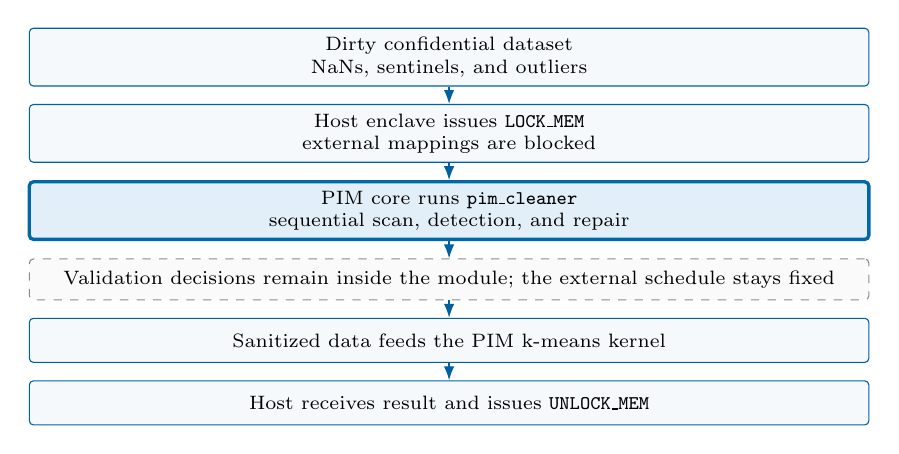
\begin{tikzpicture}[
    font=\scriptsize,
    >=Latex,
    node distance=0.22cm,
    block/.style={draw=accessblue!85!black, rounded corners=1.5pt, align=center,
        text width=0.86\columnwidth, minimum height=0.56cm, fill=accessblue!4},
    pimblock/.style={draw=accessblue!90!black, rounded corners=1.5pt, align=center,
        text width=0.86\columnwidth, minimum height=0.66cm, fill=accessblue!11,
        very thick},
    note/.style={draw=black!45, dashed, rounded corners=1.5pt, align=center,
        text width=0.86\columnwidth, minimum height=0.52cm, fill=black!2},
    arrow/.style={->, draw=accessblue!85!black, line width=0.45pt}
]
\node[block] (input) {Dirty confidential dataset\\NaNs, sentinels, and outliers};
\node[block, below=of input] (lock) {Host enclave issues \texttt{LOCK\_MEM}\\external mappings are blocked};
\node[pimblock, below=of lock] (clean) {PIM core runs \texttt{pim\_cleaner}\\sequential scan, detection, and repair};
\node[note, below=of clean] (hidden) {Validation decisions remain inside the module; the external schedule stays fixed};
\node[block, below=of hidden] (compute) {Sanitized data feeds the PIM k-means kernel};
\node[block, below=of compute] (unlock) {Host receives result and issues \texttt{UNLOCK\_MEM}};

\draw[arrow] (input) -- (lock);
\draw[arrow] (lock) -- (clean);
\draw[arrow] (clean) -- (hidden);
\draw[arrow] (hidden) -- (compute);
\draw[arrow] (compute) -- (unlock);
\end{tikzpicture}
\caption{PIM-Cleanser execution flow: host-visible operations are limited to orchestration, while data-dependent cleaning decisions execute inside the PIM module.}
\label{fig:pim_cleanser_flow}
\end{figure}

\subsection{IN-MEMORY CLEANING LOGIC}
We deploy a specialized PIM kernel, \texttt{pim\_cleaner}, directly alongside the primary workload (e.g., k-means). The cleaning kernel is designed to scan memory banks sequentially. It identifies three major categories of dirty data:
\begin{itemize}
    \item \textbf{Non-finite values:} IEEE 754 NaNs and positive or negative infinities are invalid; both signed zeros remain valid.
    \item \textbf{Null sentinel:} The implemented missing-value marker is exactly $\sentinel$, not an all-zero bit pattern.
    \item \textbf{Outliers:} Any finite value with magnitude strictly greater than the public threshold is invalid; equality at either boundary is valid.
\end{itemize}

Zero imputation is used only for normalized features. Mean imputation performs a fixed first pass to accumulate per-feature means from valid values and a fixed second pass to repair. Median and domain-aware policies remain future work. Algorithm~\ref{alg:pim_cleaner} makes the externally important rule explicit: every record is written, even when no feature changes.

\begin{algorithm}[H]
\caption{PIM-Cleanser fixed-schedule sanitization kernel}
\begin{algorithmic}[1]
\REQUIRE $M$: memory bank, public $N,D,th$, policy $p$
\ENSURE Sanitized memory bank $M$
\STATE $\mu[0..D-1]\gets 0$
\IF{$p=\textit{mean}$}
  \FOR{$i=0$ to $N-1$}
    \FOR{$d=0$ to $D-1$}
      \STATE masked-accumulate $M[i,d]$ and validity into sum/count
    \ENDFOR
  \ENDFOR
  \STATE masked-divide each public feature sum by its count
\ENDIF
\FOR{$i=0$ to $N-1$}
    \STATE $record \gets M[i]$
    \FOR{$d=0$ to $D-1$}
      \STATE $valid\gets$ finite, non-sentinel, and $|record[d]|\le th$
      \STATE $record[d]\gets\operatorname{select}(valid,record[d],\mu[d])$
    \ENDFOR
    \STATE unconditionally write $M[i]\gets record$
\ENDFOR
\end{algorithmic}
\label{alg:pim_cleaner}
\end{algorithm}

The implementation uses mask/conditional-select repair and audits generated
AArch64 assembly for feature-validity branches. More importantly for
Eq.~\eqref{eq:leakage}, validation never controls an external address, loop
bound, transfer count, or final write.

\subsection{FIXED OBSERVABLE SCHEDULE AND DRAM LOCKDOWN}
Before \texttt{pim\_cleaner} begins, the enclave issues \texttt{LOCK\_MEM}; in
the evaluated SE-PIM model, unauthorized host accesses to the protected range
are rejected until \texttt{UNLOCK\_MEM}. The PIM command carries public shape,
policy, and threshold but neither dirty indices nor a dirty count. The fixed
PIM path scans public 128~KiB actions, decomposed into 64-byte
\texttt{PIM\_ACCESS} packets, and issues unconditional writes. These mechanisms
enforce the observable-trace property in Eq.~\eqref{eq:leakage} for the defined
bus-visible observer; the threat model states the remaining channel boundaries.

\subsection{HYBRID CLEANING AND TRAFFIC SHAPING}
While full in-PIM cleaning is optimal, memory capacity constraints or complex ETL logic may require host-processor orchestration (Hybrid mode).

When host-side intervention is necessary, pulling only dirty subsets across the
bus exposes their locations. We therefore expose two distinct hybrid controls.
\texttt{hybrid-sparse} transfers only blocks containing anomalies and is an
intentionally leaky baseline. \texttt{hybrid-oblivious} scans every public
block, pads the final block to its public size, and performs the same read and
write schedule regardless of contents. Its action count is
$2\lceil B/b\rceil$ for public allocation bytes $B$ and block bytes $b$.
The oblivious candidate protects dirty-record positions under
Eq.~\eqref{eq:leakage} while retaining the public sequential layout and block
size. This matches the cleaning-specific observer defined in the threat model.

\subsection{FIXED OBSERVABLE-SCHEDULE ARGUMENT}
The observable transcript in Eq.~\eqref{eq:leakage} is the ordered record of
commands, addresses, transfer sizes and directions, issue times, status polls,
and completion visible to the attacker. Table~\ref{tab:design-modes} separates
deployment candidates from leakage
controls. \texttt{host-conditional} and \texttt{hybrid-sparse} intentionally
retain dirty-dependent writes or block selection. \texttt{host-branchless}
removes secret-dependent feature-loop branches but also reads and writes every
record; \texttt{pim-oblivious} and \texttt{hybrid-oblivious} enforce the same
rule in the protected and block-oriented paths.

\begin{table}[t]
\caption{Implemented modes and their evidence role.}
\label{tab:design-modes}
\centering\scriptsize
\begin{tabular}{lll}
\toprule
Mode & Observable schedule & Role\\
\midrule
off & no repair & workload baseline\\
host-conditional & dirty-dependent writes & leaky control\\
host-branchless & all records read/written & fixed candidate\\
pim-oblivious & fixed PIM scan/write & fixed candidate\\
hybrid-sparse & dirty-dependent blocks & leaky control\\
hybrid-oblivious & all padded blocks & fixed candidate\\
\bottomrule
\end{tabular}
\end{table}

For fixed public $P$, Algorithm~\ref{alg:pim_cleaner} executes fixed loop
bounds. Validity affects only a local conditional select, and every iteration
issues the already scheduled write. Thus command arguments, addresses, sizes,
directions, and counts are functions of $P$ alone. Fixed command completion and
equal checkpoint state make polling and $\Delta$ functions of $P$ as well,
giving Eq.~\eqref{eq:leakage}. The argument is scoped to the stated model and is
backed by artifact gates that audit AArch64 assembly, compare trace digests and
completion across equal-shape corrupted inputs, and check every output byte
against an independent reference. Publication evidence is emitted only after
all gates pass.

\section{EVALUATION}

To evaluate our proposed extension, we replicated the k-means clustering workload from the SE-PIM evaluation suite \cite{Kha:2023}. We extended the testing framework to support reproducible dataset corruption.

\subsection{METHODOLOGY}
\textbf{Evidence classes.} Host-native execution measures functional quality,
while a transparent gem5-calibrated model evaluates the full performance
matrix. Isolated native gem5 cleaning ticks anchor the cleaning parameters.
Every performance row is labeled \texttt{functional\_calibrated}, keeping the
evidence class explicit in both the CSVs and generated paper assets.

\textbf{Datasets and quality.} We use balanced labeled Gaussian mixtures,
skewed/heavy-tailed labeled mixtures, and UCI Human Activity Recognition (10,299
records, 561 normalized features, six labels) \cite{Anguita:2013}. Quality runs
cover corruption rates 0, 1, 5, 10, 20, and 40\% and seeds 7, 19, 42, 73, and
101. NaNs, infinities, the implemented $\sentinel$ marker, and public-threshold
outliers are injected at recorded positions. We report within-cluster sum of
squares (WCSS), clean-reference WCSS ratio, centroid drift after optimal
matching, normalized mutual information (NMI), remaining invalid values, and
feature-aggregation error.

\begin{table}[t]
\caption{Datasets used in the revised quality evaluation.}
\label{tab:datasets}
\centering\scriptsize
\begin{tabular}{lrrrl}
\toprule
Dataset & Records & Features & Labels & Distribution \\
\midrule
Balanced Gaussian & 131,072 & 8 & 6 & Gaussian \\
Skewed/heavy-tailed & 131,072 & 8 & 6 & skewed/$t$-tail \\
UCI HAR & 10,299 & 561 & 6 & normalized real \\
\bottomrule
\end{tabular}

\end{table}

\textbf{Performance matrix.} The calibrated matrix contains
\PerformanceRowCount{} individual rows spanning actual 4, 16, and 64~MiB
allocations, corruption rates 1, 10, and 40\%, three seeds, 4--64 features,
4--16 clusters, 1--128~KiB hybrid blocks, fixed-20-iteration k-means, and
feature-wise aggregation. Every run records its command, commits, source-tree
digest, dataset hashes, model kind, and individual result row.

\begin{table}[t]
\caption{Calibrated performance matrix.}
\label{tab:matrix}
\centering\scriptsize
\begin{tabular}{ll}
\toprule
Dimension & Values \\
\midrule
Actual size (MiB) & 4, 16, 64 \\
Corruption (\%) & 1, 10, 40 \\
Seeds & 7, 19, 42 \\
Features & 4, 8, 32, 64 \\
Clusters & 4, 8, 16 \\
Hybrid block (KiB) & 1, 4, 16, 64, 128 \\
Workloads & aggregation, fixed-20 $k$-means \\
Repair & zero, per-feature mean \\
\bottomrule
\end{tabular}

\end{table}

\subsection{REPAIR QUALITY AND PERFORMANCE}
All zero and mean policies repair every supported anomaly; clean input remains
byte-identical and a second repair is idempotent. Table~\ref{tab:quality}
quantifies the downstream utility of the repaired data.
At 10\% UCI HAR corruption, mean imputation reduces aggregation error from
0.0671 to 0.0017 and centroid drift from 2.472 to 0.795 relative to zero repair,
but NMI is slightly lower (0.546 versus 0.559). Policy selection must therefore
follow the downstream objective rather than a universal cleanliness score.

\begin{table}[t]
\caption{UCI HAR quality at 10\% corruption (five-seed means).}
\label{tab:quality}
\centering\scriptsize
\begin{tabular}{lrrrr}
\toprule
Policy & WCSS ratio & Drift & NMI & Agg. error \\
\midrule
None & -- & -- & 0.001 & -- \\
Zero & 1.040 & 2.472 & 0.559 & 0.0671 \\
Mean & 0.963 & 0.795 & 0.546 & 0.0017 \\
\bottomrule
\end{tabular}

\end{table}

Table~\ref{tab:quality-cross} extends the comparison across all three
distributions. Mean repair has much lower aggregation error on all three
datasets and lower drift on the skewed and UCI data. NMI, however, is tied on
the balanced mixture and slightly favors zero repair on UCI HAR, reinforcing
that imputation is application-specific.

\begin{table*}[t]
\caption{Quality across datasets at 10\% corruption (five-seed means).}
\label{tab:quality-cross}
\centering\scriptsize
\begin{tabular}{llrrrr}
\toprule
Dataset & Policy & WCSS ratio & Drift & NMI & Agg. error \\
\midrule
Balanced Gaussian & Zero & 1.046 & 0.193 & 0.835 & 0.0710 \\
Balanced Gaussian & Mean & 1.041 & 0.188 & 0.835 & 0.0070 \\
Skewed/heavy-tailed & Zero & 0.962 & 0.336 & 0.593 & 0.0703 \\
Skewed/heavy-tailed & Mean & 0.944 & 0.112 & 0.611 & 0.0008 \\
UCI HAR & Zero & 1.040 & 2.472 & 0.559 & 0.0671 \\
UCI HAR & Mean & 0.963 & 0.795 & 0.546 & 0.0017 \\
\bottomrule
\end{tabular}

\end{table*}

Figure~\ref{fig:pim_cleaning} presents the performance--quality policy
tradeoff. The bars are calibrated
incremental overhead for the selected 4~MiB fixed-20 k-means configuration; the
line is host-native UCI HAR aggregation error at 10\% corruption. They are
reported on separate axes because they represent complementary evidence
classes. Mean repair reduces aggregation error by 97.5\% relative to zero
repair while retaining sub-0.12\% estimated incremental overhead.

\begin{figure}[t]
\centering
\begin{tikzpicture}
\begin{axis}[
  width=0.88\columnwidth,height=4.0cm,
  ybar,bar width=15pt,
  xmin=0.5,xmax=2.5,xtick={1,2},xticklabels={Zero,Mean},
  ylabel={Calibrated overhead (\%)},ymin=0,ymax=0.14,
  grid=major,axis y line*=left,
  legend style={font=\tiny,at={(0.02,0.98)},anchor=north west},
  tick label style={font=\scriptsize},label style={font=\scriptsize}]
\addplot+[fill=accessblue!55,draw=accessblue] table[x=policy_id,y=overhead_pct,col sep=comma]
  {paper/generated/policy_tradeoff.csv};
\addlegendentry{Overhead}
\end{axis}
\begin{axis}[
  width=0.88\columnwidth,height=4.0cm,
  xmin=0.5,xmax=2.5,xtick=\empty,
  ylabel={Aggregation error},ymin=0,ymax=0.075,
  axis y line*=right,axis x line=none,
  legend style={font=\tiny,at={(0.98,0.98)},anchor=north east},
  tick label style={font=\scriptsize},label style={font=\scriptsize}]
\addplot+[red!75!black,mark=diamond*,thick] table[x=policy_id,y=aggregation_error,col sep=comma]
  {paper/generated/policy_tradeoff.csv};
\addlegendentry{Aggregation error}
\end{axis}
\end{tikzpicture}
\caption{Performance--quality policy comparison: calibrated overhead and
host-native UCI HAR aggregation error.}
\label{fig:pim_cleaning}
\end{figure}

For the selected 4~MiB, 32-feature, $K=8$, fixed-20 k-means configuration,
the calibrated model estimates $0.048495\%$ incremental overhead for
PIM-oblivious zero imputation and $0.117989\%$ for mean imputation. These
estimates are parameterized using isolated native gem5 cleaning measurements;
the resulting full-workload matrix explores how policy and public shape affect
cost while preserving a traceable evidence boundary.

Figure~\ref{fig:quality_sensitivity} quantifies corruption-rate sensitivity.
Mean repair removes every supported invalid value at every rate. WCSS ratio and
NMI decline gradually as less original information remains, capturing the
expected statistical limit of imputation rather than a repair failure.

\begin{figure}[t]
\centering
\begin{tikzpicture}
\begin{axis}[
  width=\columnwidth,height=3.8cm,
  xlabel={Corruption (\%)}, ylabel={Metric},
  ymin=0.35,ymax=1.05, grid=major,
  legend style={font=\tiny,at={(0.5,-0.30)},anchor=north,legend columns=2},
  tick label style={font=\scriptsize},label style={font=\scriptsize}]
\addplot+[mark=*,thick] table[x=rate_pct,y=wcss_ratio,col sep=comma]
  {paper/generated/quality_uci_mean.csv};
\addlegendentry{WCSS ratio}
\addplot+[mark=square*,thick] table[x=rate_pct,y=nmi,col sep=comma]
  {paper/generated/quality_uci_mean.csv};
\addlegendentry{NMI}
\end{axis}
\end{tikzpicture}
\caption{Mean-imputation quality sensitivity on UCI HAR across corruption
rates.}
\label{fig:quality_sensitivity}
\end{figure}

\subsection{HYBRID MODE SCALING}
Figure~\ref{fig:hybrid_scaling} reports execution time and throughput for the
selected 4~MiB,
32-feature, $K=8$, mean-imputation k-means case at 10\% corruption, averaged
over seeds 7, 19, and 42. Increasing the public block size from 1 to 128~KiB
reduces calibrated runtime from 0.791 to 0.059~s and raises throughput from 5.29
to 158.51~MiB/s. Larger blocks therefore amortize controlled-access setup
effectively while preserving the hybrid-oblivious schedule.

\begin{figure}[t]
\centering
\begin{tikzpicture}
\begin{axis}[
  width=0.90\columnwidth,height=4.0cm,
  xlabel={DMA block (KiB)},ylabel={Calibrated runtime (s)},
  ymin=0,grid=major,axis y line*=left,
  legend style={font=\tiny,at={(0.02,0.98)},anchor=north west},
  tick label style={font=\scriptsize},label style={font=\scriptsize}]
\addplot+[mark=*,thick] table[x=block_kib,y=hybrid_oblivious_runtime_sec,col sep=comma]
 {paper/generated/hybrid_block.csv};
\addlegendentry{Runtime}
\end{axis}
\begin{axis}[
  width=0.90\columnwidth,height=4.0cm,
  xmin=0,xmax=135,xtick=\empty,
  ylabel={Throughput (MiB/s)},ymin=0,
  axis y line*=right,axis x line=none,
  legend style={font=\tiny,at={(0.98,0.98)},anchor=north east},
  tick label style={font=\scriptsize},label style={font=\scriptsize}]
\addplot+[red!75!black,mark=square*,thick] table[x=block_kib,y=hybrid_oblivious_throughput_mib_s,col sep=comma]
 {paper/generated/hybrid_block.csv};
\addlegendentry{Throughput}
\end{axis}
\end{tikzpicture}
\caption{Calibrated hybrid-oblivious runtime and throughput versus public block
size.}
\label{fig:hybrid_scaling}
\end{figure}

Figure~\ref{fig:phase_breakdown} explains the scaling result by separating the
modeled cycle components. Controlled-access setup dominates small hybrid
blocks, and larger blocks amortize that cost. The PIM-oblivious bar is almost
entirely the fixed k-means workload, explaining its small calibrated
incremental overhead.

\begin{figure}[t]
\centering
\begin{tikzpicture}
\begin{axis}[
  width=\columnwidth,height=4.1cm,
  ybar stacked,bar width=11pt,
  xmin=0.5,xmax=4.5,xtick={1,2,3,4},
  xticklabels={PIM,Hyb. 1K,Hyb. 16K,Hyb. 128K},
  ylabel={Calibrated time (s)},ymin=0,grid=major,
  legend style={font=\tiny,at={(0.5,-0.34)},anchor=north,legend columns=4},
  tick label style={font=\tiny},label style={font=\scriptsize}]
\addplot+[fill=accessblue!25,draw=accessblue!60] table[x=case_id,y=scan_sec,col sep=comma]
  {paper/generated/phase_breakdown.csv};
\addlegendentry{Scan}
\addplot+[fill=green!45,draw=green!50!black] table[x=case_id,y=clean_sec,col sep=comma]
  {paper/generated/phase_breakdown.csv};
\addlegendentry{Clean}
\addplot+[fill=orange!60,draw=orange!80!black] table[x=case_id,y=access_sec,col sep=comma]
  {paper/generated/phase_breakdown.csv};
\addlegendentry{Access}
\addplot+[fill=gray!60,draw=gray!80] table[x=case_id,y=workload_sec,col sep=comma]
  {paper/generated/phase_breakdown.csv};
\addlegendentry{Workload}
\end{axis}
\end{tikzpicture}
\caption{Timing-component breakdown for mean-imputation k-means.
Hybrid labels denote public block size.}
\label{fig:phase_breakdown}
\end{figure}

Leakage is tested directly rather than inferred from mode names. Across all
1,008 equal-public-shape groups, fixed candidates have one modeled observable
trace; host-conditional and hybrid-sparse controls vary as expected. As shown in Figure~\ref{fig:leakage}, in a representative aggregation case, PIM-oblivious and hybrid-oblivious completion are constant across corruption, whereas the leaky controls' completion changes
with dirty density. The trace includes transfers, bytes, padding, poll
count, and completion, so sequential addresses alone are insufficient to pass.

\begin{figure}[t]
\centering
\begin{tikzpicture}
\begin{semilogyaxis}[
 width=\columnwidth,height=4.0cm,
 xlabel={Corruption (\%)},ylabel={Cleaning completion (modeled cycles)},
 grid=major,legend style={font=\tiny,at={(0.5,-0.32)},anchor=north,legend columns=2},
 tick label style={font=\scriptsize},label style={font=\scriptsize}]
\addplot+[mark=*,thick] table[x=rate_pct,y=hostconditional_cycles,col sep=comma]
 {paper/generated/leakage.csv};
\addlegendentry{host-conditional}
\addplot+[mark=triangle*,thick] table[x=rate_pct,y=hybridsparse_cycles,col sep=comma]
 {paper/generated/leakage.csv};
\addlegendentry{hybrid-sparse}
\addplot+[mark=square*,thick] table[x=rate_pct,y=pimoblivious_cycles,col sep=comma]
 {paper/generated/leakage.csv};
\addlegendentry{pim-oblivious}
\addplot+[mark=diamond*,thick] table[x=rate_pct,y=hybridoblivious_cycles,col sep=comma]
 {paper/generated/leakage.csv};
\addlegendentry{hybrid-oblivious}
\end{semilogyaxis}
\end{tikzpicture}
\caption{Empirical leakage control: fixed schedules remain horizontal while
leaky controls expose dirty-density-dependent completion.}
\label{fig:leakage}
\end{figure}

\begin{table}[t]
\caption{Calibrated observable-schedule outcome by mode.}
\label{tab:modes}
\centering\scriptsize
\begin{tabular}{lrrl}
\toprule
Mode & Rows & Schedule result & Evidence role \\
\midrule
off & 1,296 & none & baseline \\
host-conditional & 1,296 & varies & leaky control \\
host-branchless & 1,296 & equal & fixed candidate \\
pim-oblivious & 1,296 & equal & fixed candidate \\
hybrid-sparse & 6,480 & varies & leaky control \\
hybrid-oblivious & 6,480 & equal & fixed candidate \\
\bottomrule
\end{tabular}

\end{table}

\begin{table}[t]
\caption{Calibrated overhead at 10\% corruption (4~MiB, 32 features,
$K=8$, mean repair, fixed-20 k-means; 16~KiB hybrid blocks).}
\label{tab:cost}
\centering\scriptsize
\begin{tabular}{lr}
\toprule
Mode & Overhead (\%)\\
\midrule
off & 0.0\\
host-conditional & 9560.3\\
host-branchless & 17435.6\\
pim-oblivious & 0.117989\\
hybrid-sparse & 190.2\\
hybrid-oblivious & 192.4\\
\bottomrule
\end{tabular}
\end{table}

The host-mode values quantify the cost of repeated controlled-access setup on
small records. PIM batching removes those host transactions.
Changing the device formula, burst size, cleaner parallelism, or downstream
arithmetic rate requires recalibration and regeneration rather than reuse of
these percentages.

\subsection{SCOPE AND REPRODUCIBILITY}
The performance study targets the event-driven legacy SE-PIM ARM gem5 model.
The full-workload values are calibrated estimates anchored by isolated native
cleaning timing. The artifact also provides a separately gated direct native
end-to-end path; its evidence is promoted only after its provenance,
correctness, trace, timing, and regression checks pass. Absolute values depend
on the modeled memory system, checkpoint, device constants, and assumed
16-core arithmetic throughput, so a different platform requires recalibration.
Zero repair targets normalized features, while mean repair may alter
correlations. Median and domain-aware imputation, categorical repair,
duplicates, schema repair, and power/EM or internal PIM-core channels define
useful extensions beyond the present study.

Each run uses a unique identifier and records commands, commits, source digest,
dataset hashes, seeds, timestamps, and model kind. The checksum-pinned UCI
converter emits label sidecars and complete metadata. The release artifact
contains canonical individual CSV rows, generated paper inputs, source, and a
clean-extraction verifier. This separation lets every reported value be traced
to its evidence class and regenerated from a clean extraction.

\section{CONCLUSION}
PIM-Cleanser addresses the clean-data assumption in confidential PIM by integrating
sanitization directly into the protected SE-PIM execution path. Its fixed modes
repair every supported anomaly through schedules determined solely by public
shape. Across 1,008 equal-public-shape groups, these modes maintain identical
modeled observable traces, while explicit leakage controls exhibit the expected
dirty-density dependence. Host-native quality experiments demonstrate the
utility and statistical tradeoffs of zero and mean repair across synthetic and
real data. The gem5-calibrated model estimates only $0.048495\%$ incremental
overhead for zero repair and $0.117989\%$ for mean repair in the selected
k-means configuration. Together, these results establish fixed-schedule data
repair under the evaluated observer with low estimated performance cost.
Direct gem5 events \cite{LowePower2020} confirm a fixed native cleaning
transcript for the evaluated public shapes. The artifact's separation of
evidence, negative controls, and reproducibility gates is as important as
the mechanism it evaluates.

\section{LIMITATIONS}
The native device is a gem5 event model evaluated with an older ARM
full-system bundle, not real PIM silicon. Absolute timing depends on its DMA
latencies, CPU model, memory configuration, and checkpoint. The large matrix is
calibrated, and its arithmetic throughput is an assumption. We therefore avoid
combining the two evidence types into a single measured speedup and make no
direct native end-to-end overhead claim.

Mean imputation preserves feature aggregates much better in our data, but can
distort correlations and clusters and is not always appropriate. Zero repair
is justified only for normalized features. Median, model-based, and
domain-aware repair; categorical data; duplicate detection; and schema repair
remain future work. The evaluated transcript also excludes PIM-core power,
cache, and internal branch leakage. Formal noninterference in RTL and
measurement on hardware are necessary before deployment claims.

\section*{DATA AVAILABILITY}
The artifacts supporting this paper are released at
\href{https://github.com/wafaa2026/se-pim-data-cleansing}{GitHub:
wafaa2026/se-pim-data-cleansing}. The repository includes source code,
dataset-generation and UCI conversion tools, canonical result rows, manifests,
generated paper inputs, and a clean-extraction reproduction script.

\balance
\begin{thebibliography}{00}

\bibitem{Mutlu:2019} O. Mutlu \textit{et al.}, ``Processing data where it makes sense: Enabling in-memory computation,'' \textit{Microprocessors and Microsystems}, vol. 67, pp. 28--41, 2019.

\bibitem{Kha:2023} K. D. Duy and H. Lee, ``SE-PIM: In-Memory Acceleration of Data-Intensive Confidential Computing,'' \textit{IEEE Transactions on Cloud Computing}, vol. 11, no. 3, pp. 2473--2487, July--Sept. 2023, doi: 10.1109/TCC.2022.3207145.

\bibitem{Schelter:2018} S. Schelter, D. Lange, P. Schmidt, M. Celikel, F. Biessmann, and A. Grafberger, ``Automating Large-Scale Data Quality Verification,'' \textit{Proc. VLDB Endowment}, vol. 11, no. 12, pp. 1781--1794, Aug. 2018, doi: 10.14778/3229863.3229867.

\bibitem{Qi:2021} Z. Qi, H. Wang, and A.-J. Wang, ``Impacts of Dirty Data on Classification and Clustering Models: An Experimental Evaluation,'' \textit{Journal of Computer Science and Technology}, vol. 36, no. 4, pp. 806--821, 2021, doi: 10.1007/s11390-021-1344-6.

\bibitem{Sambasivan:2021} N. Sambasivan, S. Kapania, H. Highfill, D. Akrong, P. K. Paritosh, and L. M. Aroyo, ``Everyone Wants to Do the Model Work, Not the Data Work: Data Cascades in High-Stakes AI,'' in \textit{Proc. CHI Conference on Human Factors in Computing Systems}, 2021, pp. 1--15, doi: 10.1145/3411764.3445518.

\bibitem{Xu:2015} Y. Xu, W. Cui, and M. Peinado, ``Controlled-Channel Attacks: Deterministic Side Channels for Untrusted Operating Systems,'' in \textit{Proc. IEEE Symp. Security and Privacy (S\&P)}, San Jose, CA, May 2015.

\bibitem{Lee:2017} S. Lee, M.-W. Shih, P. Gera, T. Kim, H. Kim, and M. Peinado, ``Inferring Fine-Grained Control Flow Inside SGX Enclaves with Branch Shadowing,'' in \textit{Proc. USENIX Security Symposium}, 2017, pp. 557--574.

\bibitem{Fernandes:2023} A. A. A. Fernandes, M. Koehler, N. Konstantinou, P. Pankin, N. W. Paton, and R. Sakellariou, ``Data Preparation: A Technological Perspective and Review,'' \textit{SN Computer Science}, vol. 4, no. 4, 2023, doi: 10.1007/s42979-023-01828-8.

\bibitem{Chawla:2013} S. Chawla and A. Gionis, ``k-means--: A Unified Approach to Clustering and Outlier Detection,'' in \textit{Proc. SIAM International Conference on Data Mining}, 2013, pp. 189--197, doi: 10.1137/1.9781611972832.21.

\bibitem{Im:2020} S. Im, M. M. Qaem, B. Moseley, X. Sun, and R. Zhou, ``Fast Noise Removal for k-Means Clustering,'' in \textit{Proc. International Conference on Artificial Intelligence and Statistics}, PMLR, vol. 108, pp. 456--466, 2020.

\bibitem{Gruss:2016} D. Gruss, C. Maurice, A. Fogh, M. Lipp, and S. Mangard, ``Prefetch Side-Channel Attacks: Bypassing SMAP and Kernel ASLR,'' in \textit{Proc. ACM SIGSAC Conference on Computer and Communications Security (CCS)}, Vienna, Austria, Oct. 2016, pp. 368--379, doi: 10.1145/2976749.2978356.

\bibitem{Chen:2023} Z. Chen, S. Tan, U. Chajewska, C. Rudin, and R. Caruna, ``Missing Values and Imputation in Healthcare Data: Can Interpretable Machine Learning Help?'' in \textit{Proc. Conference on Health, Inference, and Learning}, PMLR, vol. 209, pp. 86--99, 2023.

\bibitem{Goldreich:1996} O. Goldreich and R. Ostrovsky, ``Software Protection and Simulation on Oblivious RAMs,'' \textit{Journal of the ACM}, vol. 43, no. 3, pp. 431--473, 1996.

\bibitem{Eskandarian:2019} S. Eskandarian and M. Zaharia, ``ObliDB: Oblivious query processing for secure databases,'' \textit{Proc. VLDB Endowment}, vol. 13, no. 2, pp. 169--183, 2019, doi: 10.14778/3364324.3364331.

\bibitem{GomezLuna:2021} J. G\'omez-Luna, I. El Hajj, I. Fernandez, C. Giannoula, G. F. Oliveira, and O. Mutlu, ``Benchmarking memory-centric computing systems: Analysis of real processing-in-memory hardware,'' \textit{arXiv:2110.01709}, 2021.

\bibitem{Arafin:2020} M. T. Arafin and Z. Lu, ``Security challenges of processing-in-memory systems,'' in \textit{Proc. ACM Great Lakes Symp. VLSI}, 2020, pp. 229--234, doi: 10.1145/3386263.3411365.

\bibitem{Anguita:2013} D. Anguita, A. Ghio, L. Oneto, X. Parra, and J. L. Reyes-Ortiz, ``A public domain dataset for human activity recognition using smartphones,'' in \textit{Proc. ESANN}, 2013, pp. 437--442.

\bibitem{LowePower2020} J. Lowe-Power \emph{et al.}, ``The gem5 simulator: Version 20.0+,'' \emph{arXiv:2007.03152}, 2020.

\end{thebibliography}

\end{document}
